\section{Расчет коэффициента обратной связи, сравнение с результатами Дваера}\label{sec:thunderstorm/rdfm}

Несмотря на то что в хороших условиях в лавине убегающих электронов может быть сгенерировано более миллиона дополнительных электронов, это не объясняет большие потоки гамма-квантов в TGF, а также не дает объяснения как связанны между собой процессы с высокоэнергетичными частицами и разряды молнии. Одним из вариантов модификации теории Гуревича, является построение на её основе модели с обратной связью (ОС). Джозеф Дуайер в работе~\cite{dwyer2003fundamental} предложил рассмотреть два механизма которые могут привести к возникновению обратной связи: гамма обратная связь возникает за счет того что не смотря на то что рождаемые убегающими электронами гамма-квант имеют начальный импульс сонаправленный с направление движения лавины, часть из них в результате рассеяния может в итоге оказаться в части облака в котором начиналась лавина и выбить там электрон, который станет новым затравочным электроном, позитронная обратная связь возникает за счет конверсии гамма-квантов электрон-позитронные пары, при этом позитрон имеет шанс развернутся в электрическом поле и начать ускорятся против направления распространения лавины, выбивая вторичные электроны, которые опять же имеют шанс развернутся в электрическом поле и стать новым затравочным электроном. Рисунок проведенного мною моделирования, иллюстрирует описание позитронной обратной связи: красные треки отображают лавину убегающих электронов, зеленные треки тормозные гамма-кванты, синий трек показывает позитрон обратной связи, который как мы видим создает новые затравочные электроны (которые правда не создают новую лавину). Механизмы описанные Дуайером должны работать в широком диапазоне атмосферных условий, однако являются вероятностными и возникает вопрос насколько значителен вклад этих механизмов в развитие лавин убегающих электронов.

\begin{figure}[ph!]
    \begin{center}
        \includegraphics[width=\linewidth]{thunderstorm/ayss_2018_art/10_dwyer.pdf}
        \caption{Распространение лавины убегающих электронов, красные треки --- электроны, зеленые треки --- гамма-кванты, синий трек --- позитрон.}
    \end{center}
    \label{fig:storm:dwyer}
\end{figure}

В работе~\cite{dwyer2003fundamental} приводятся результаты моделирования при нормальных условиях исследующие при каких соотношениях длины области с электрическим полем и величины поля может возникать обратная связь. Для проверки данных результатов было проведено собственное моделирование, состоящее из двух частей моделирование рождения вторичных электронов и расчет вероятности разворота электронов электрическом поле. 

\begin{figure}[ph!]
    \begin{center}
        \begin{minipage}[h]{0.49\linewidth}
            \center{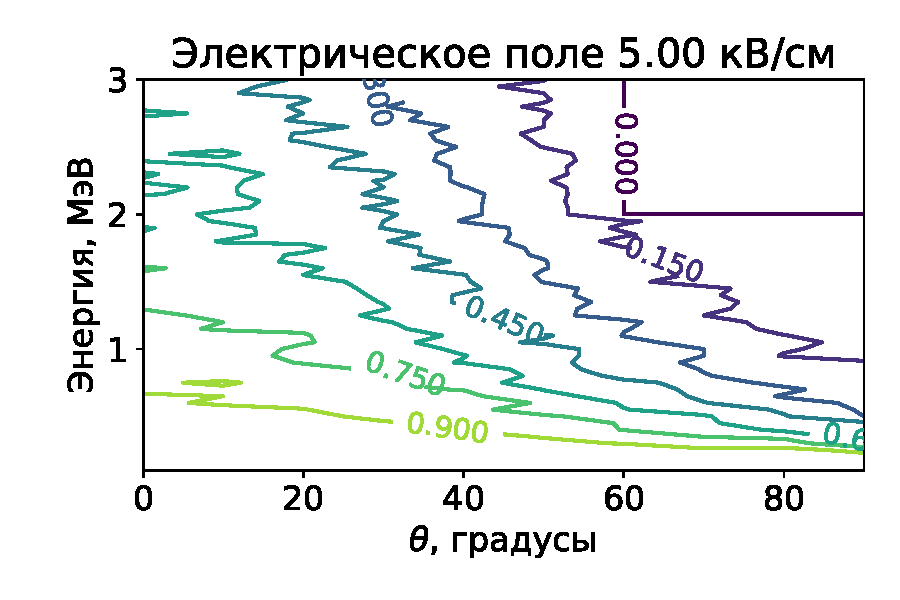
\includegraphics[width=\linewidth]{thunderstorm/rdfm/reverse_5_00.pdf} \\ а)}
        \end{minipage}
        \hfill
        \begin{minipage}[h]{0.49\linewidth}
            \center{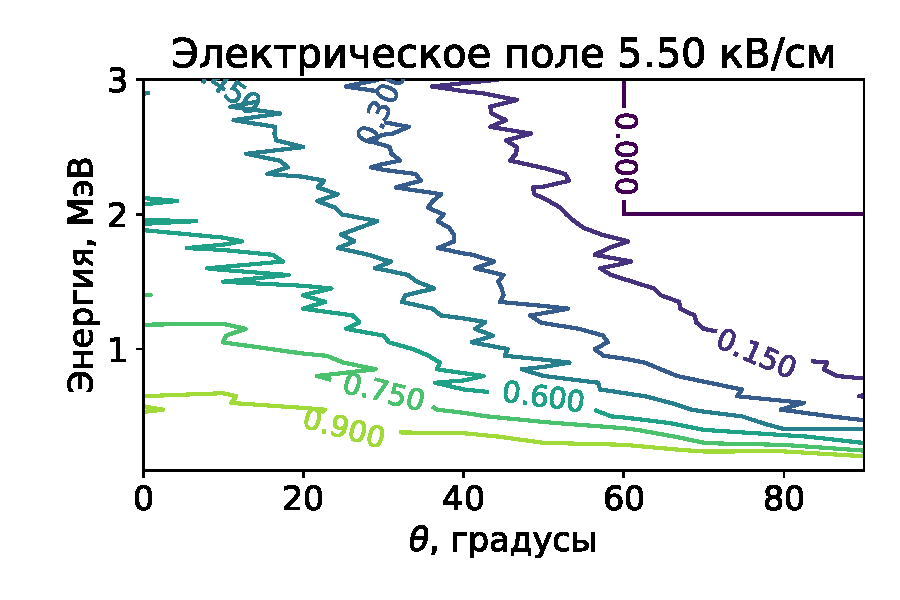
\includegraphics[width=\linewidth]{thunderstorm/rdfm/reverse_5_50.pdf} \\ б)}
        \end{minipage}
        \vfill
        \begin{minipage}[h]{0.49\linewidth}
            \center{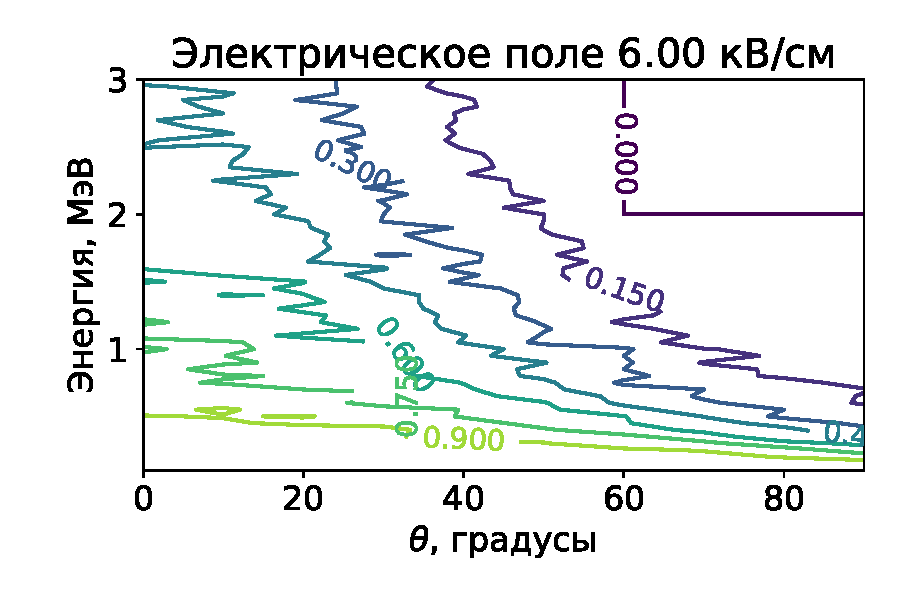
\includegraphics[width=\linewidth]{thunderstorm/rdfm/reverse_6_00.pdf} \\ в)}
        \end{minipage}
        \hfill
        \begin{minipage}[h]{0.49\linewidth}
            \center{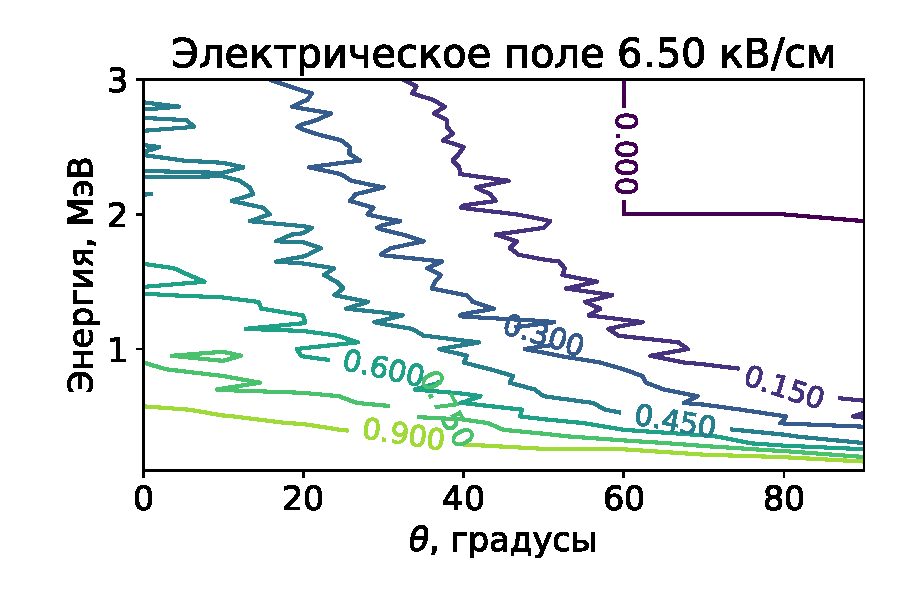
\includegraphics[width=\linewidth]{thunderstorm/rdfm/reverse_6_50.pdf} \\ г)}
        \end{minipage}
        \vfill
        \begin{minipage}[h]{0.49\linewidth}
            \center{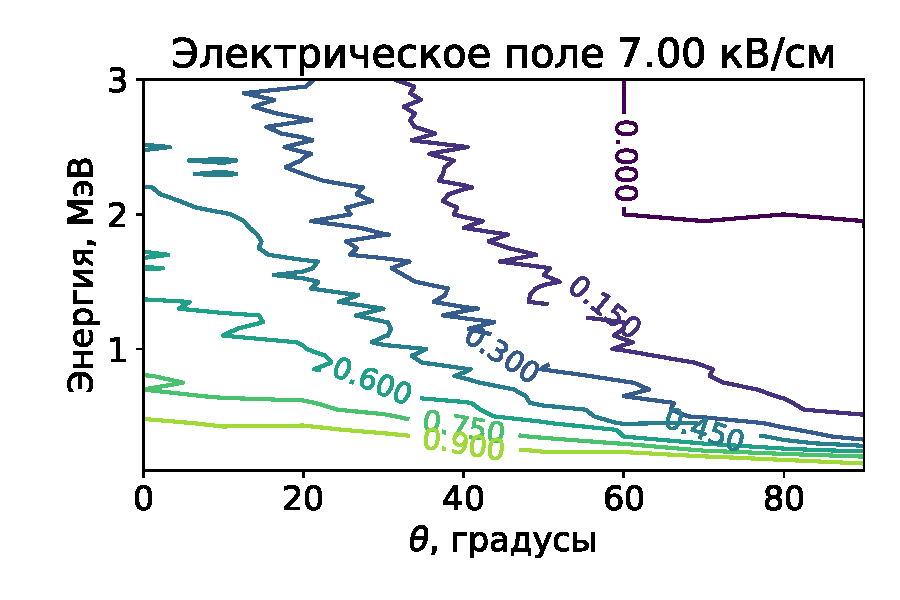
\includegraphics[width=\linewidth]{thunderstorm/rdfm/reverse_7_00.pdf} \\ д)}
        \end{minipage}
        \hfill
        \begin{minipage}[h]{0.49\linewidth}
            \center{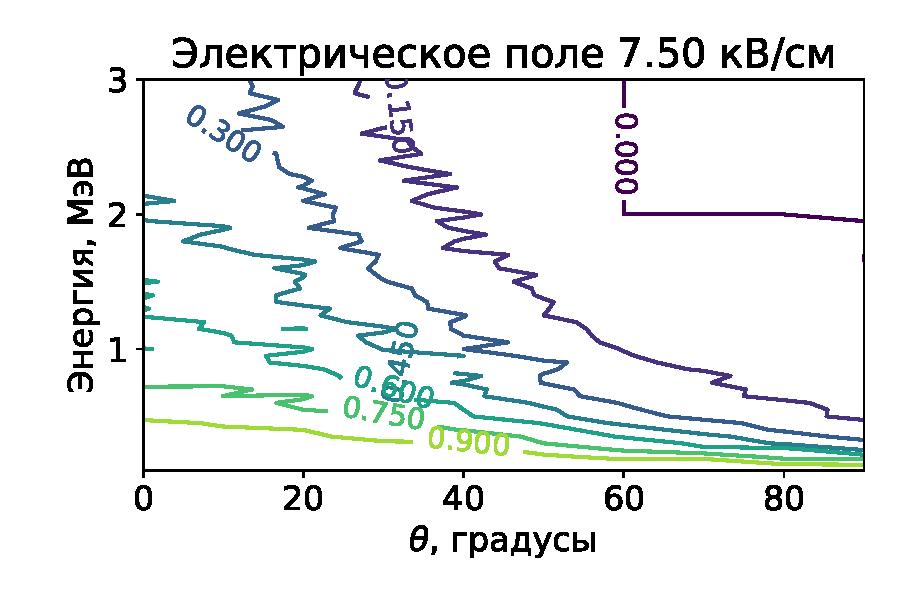
\includegraphics[width=\linewidth]{thunderstorm/rdfm/reverse_7_50.pdf} \\ е)}
        \end{minipage}
        \caption{Разворот электрона}
    \end{center}
    \label{fig:storm:reverse_nc_1}
\end{figure}
\begin{figure}[ph!]
    \begin{center}
        \begin{minipage}[h]{0.49\linewidth}
            \center{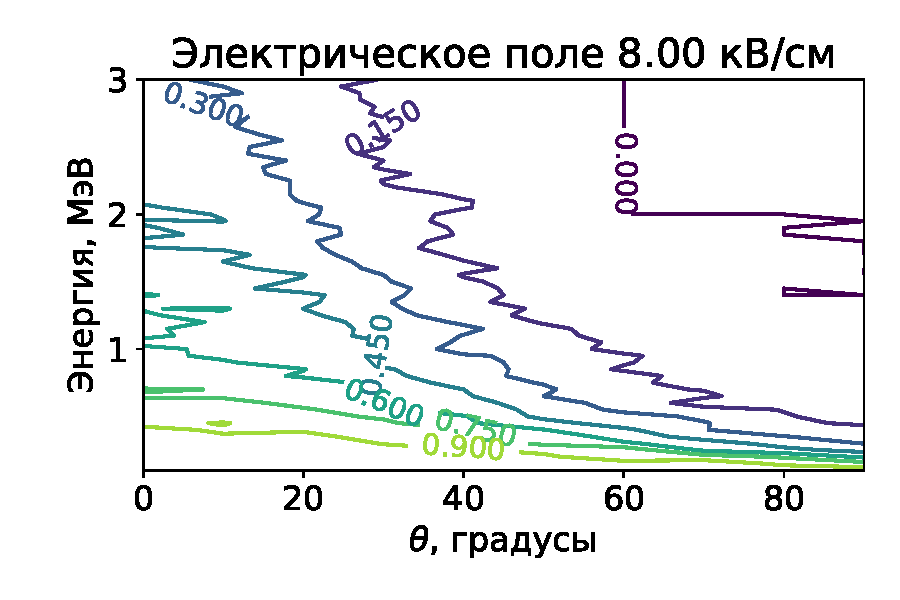
\includegraphics[width=\linewidth]{thunderstorm/rdfm/reverse_8_00.pdf} \\ ж)}
        \end{minipage}
        \hfill
        \begin{minipage}[h]{0.49\linewidth}
            \center{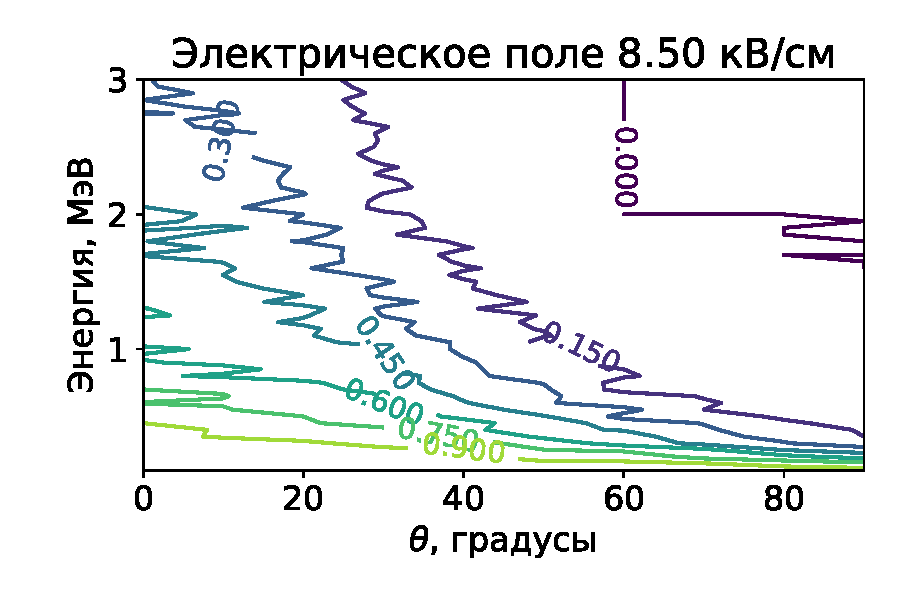
\includegraphics[width=\linewidth]{thunderstorm/rdfm/reverse_8_50.pdf} \\ з)}
        \end{minipage}    
        \vfill
        \begin{minipage}[h]{0.49\linewidth}
            \center{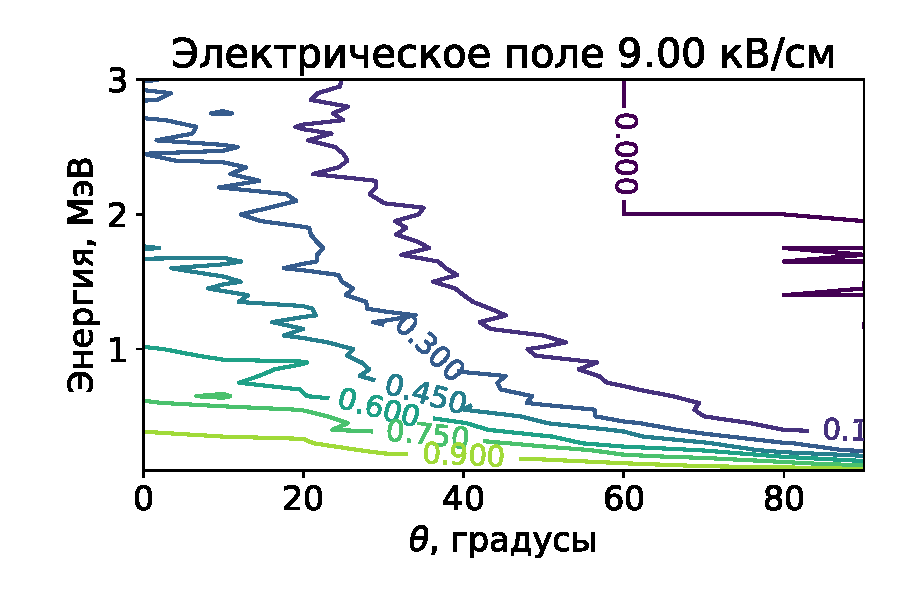
\includegraphics[width=\linewidth]{thunderstorm/rdfm/reverse_9_00.pdf} \\ и)}
        \end{minipage}
        \hfill
        \begin{minipage}[h]{0.49\linewidth}
            \center{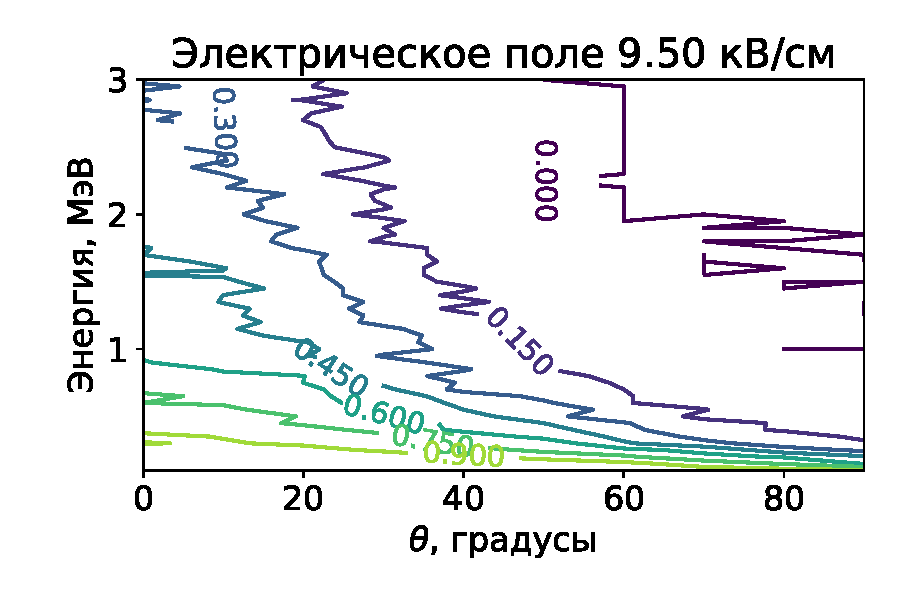
\includegraphics[width=\linewidth]{thunderstorm/rdfm/reverse_9_50.pdf} \\ к)}
        \end{minipage} 
        \vfill
        \begin{minipage}[h]{0.49\linewidth}
            \center{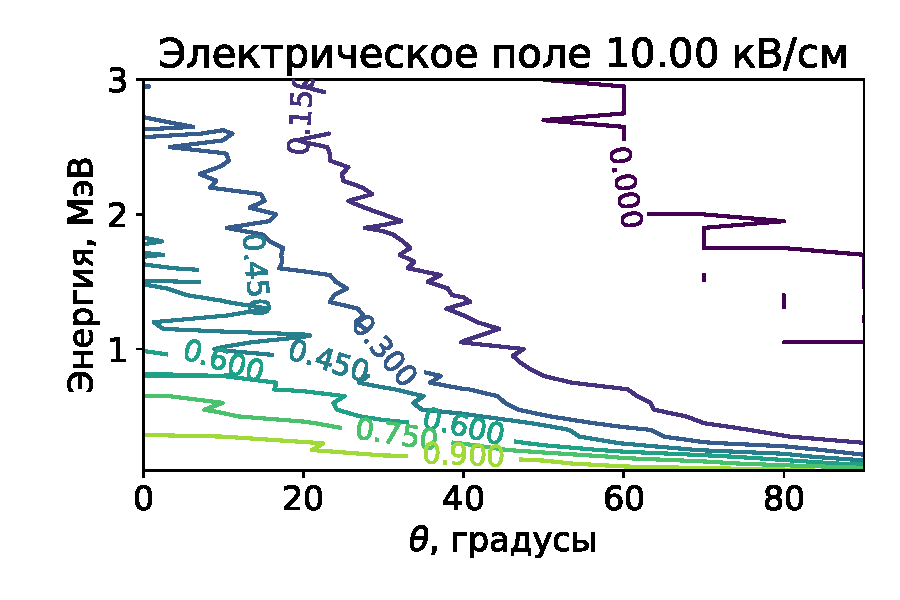
\includegraphics[width=\linewidth]{thunderstorm/rdfm/reverse_10_00.pdf} \\ л)}
        \end{minipage}
        \caption{Разворот электрона}
    \end{center}
    \label{fig:storm:reverse_nc_2}
\end{figure}


\begin{figure}[ph!]
    \begin{center}
        \begin{minipage}[h]{0.49\linewidth}
            \center{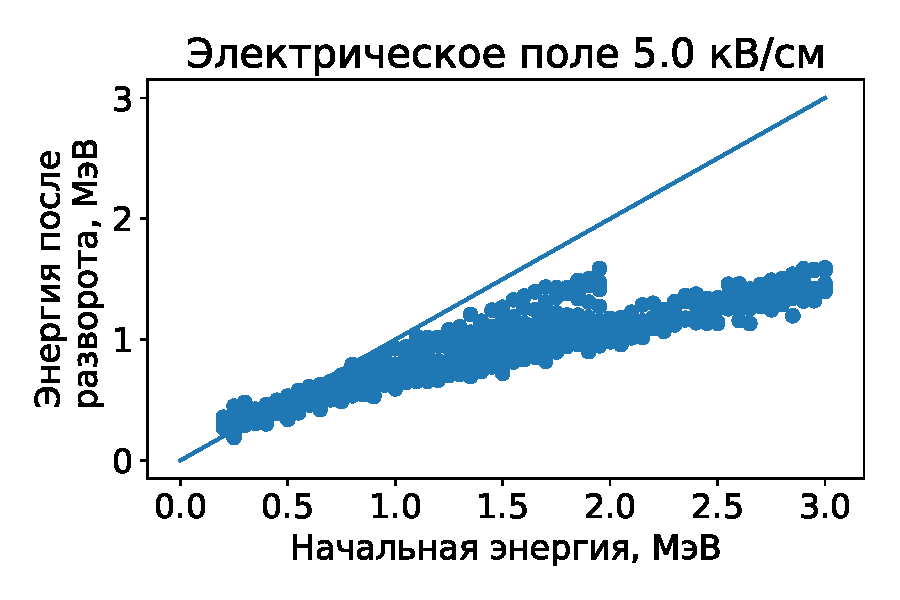
\includegraphics[width=\linewidth]{thunderstorm/rdfm/reverse_energy_5_0.pdf} \\ а)}
        \end{minipage}
        \hfill
        \begin{minipage}[h]{0.49\linewidth}
            \center{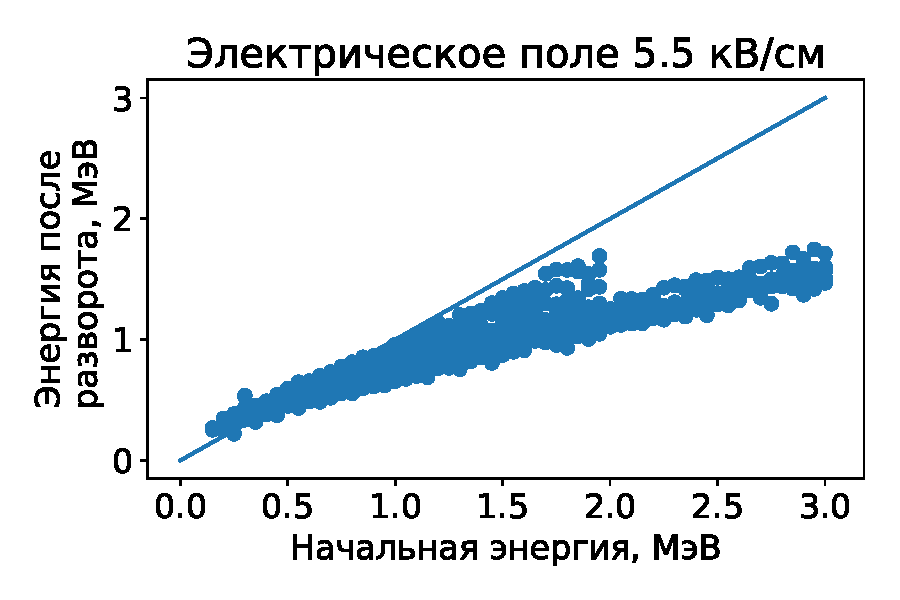
\includegraphics[width=\linewidth]{thunderstorm/rdfm/reverse_energy_5_5.pdf} \\ б)}
        \end{minipage}
        \vfill
        \begin{minipage}[h]{0.49\linewidth}
            \center{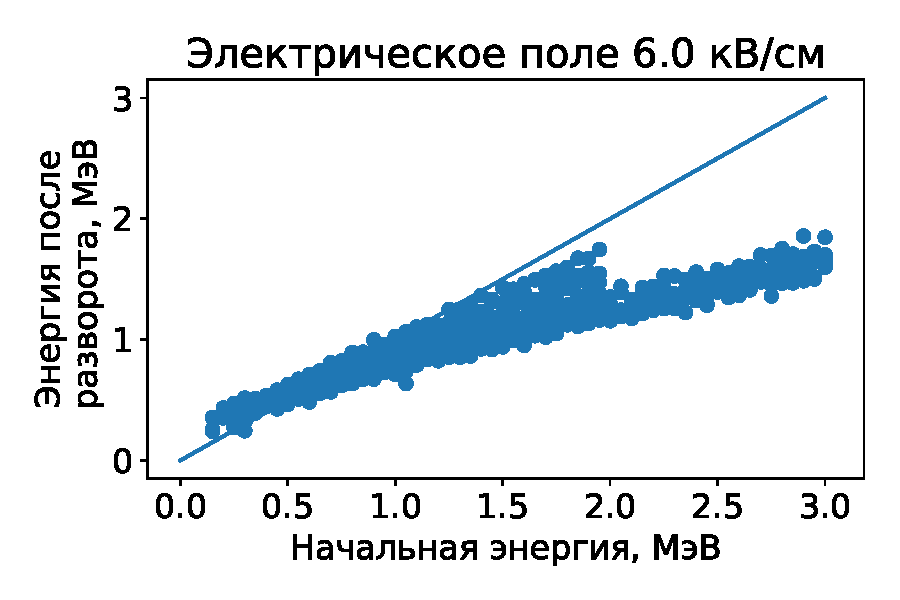
\includegraphics[width=\linewidth]{thunderstorm/rdfm/reverse_energy_6_0.pdf} \\ в)}
        \end{minipage}
        \hfill
        \begin{minipage}[h]{0.49\linewidth}
            \center{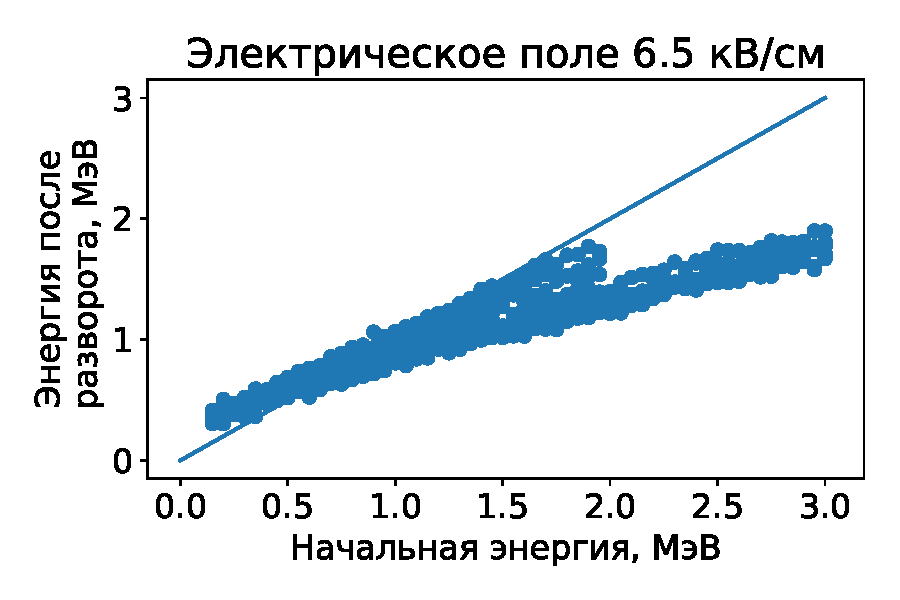
\includegraphics[width=\linewidth]{thunderstorm/rdfm/reverse_energy_6_5.pdf} \\ г)}
        \end{minipage}
        \vfill
        \begin{minipage}[h]{0.49\linewidth}
            \center{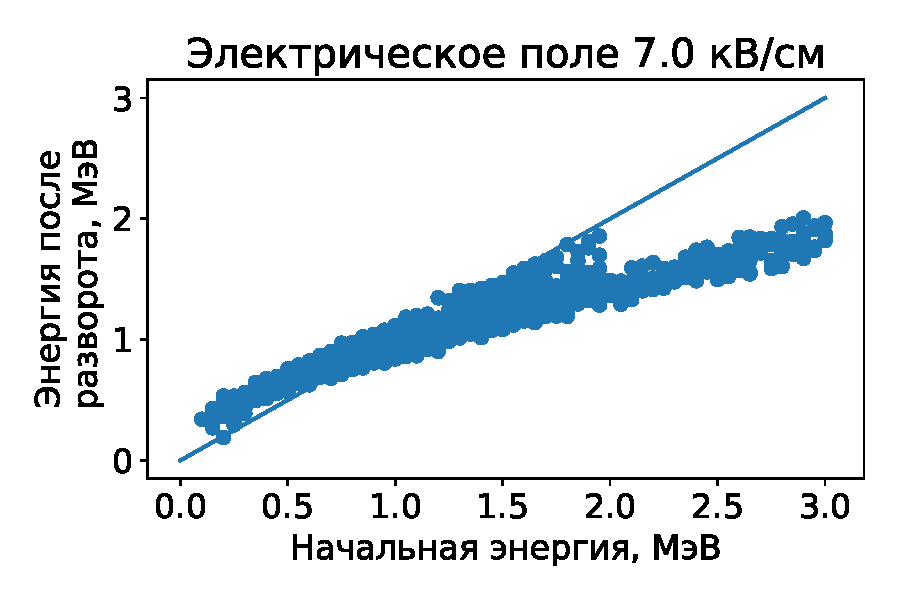
\includegraphics[width=\linewidth]{thunderstorm/rdfm/reverse_energy_7_0.pdf} \\ д)}
        \end{minipage}
        \hfill
        \begin{minipage}[h]{0.49\linewidth}
            \center{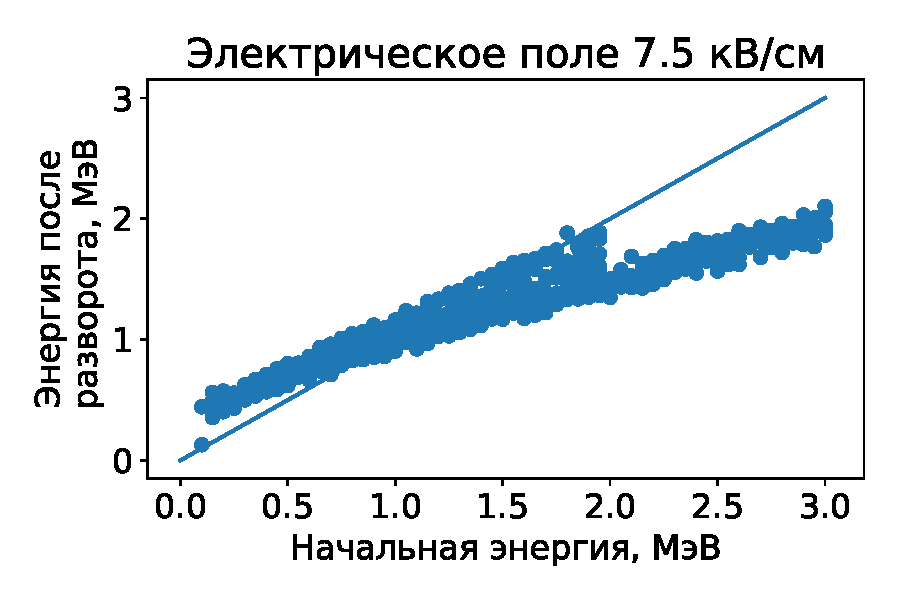
\includegraphics[width=\linewidth]{thunderstorm/rdfm/reverse_energy_7_5.pdf} \\ е)}
        \end{minipage}
        \caption{Разворот электрона}
    \end{center}
    \label{fig:storm:reverse_energy_nc_1}
\end{figure}
\begin{figure}[ph!]
    \begin{center}
        \begin{minipage}[h]{0.49\linewidth}
            \center{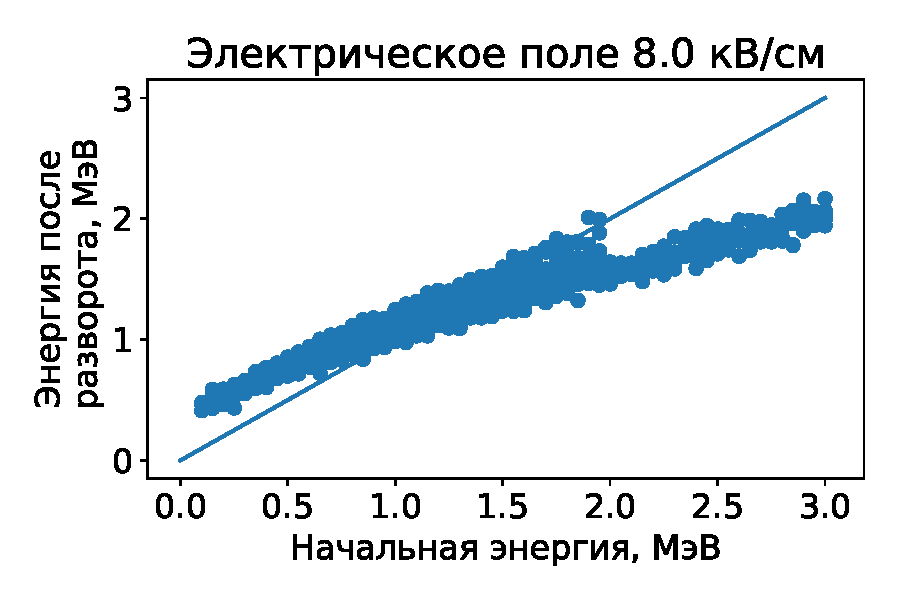
\includegraphics[width=\linewidth]{thunderstorm/rdfm/reverse_energy_8_0.pdf} \\ ж)}
        \end{minipage}
        \hfill
        \begin{minipage}[h]{0.49\linewidth}
            \center{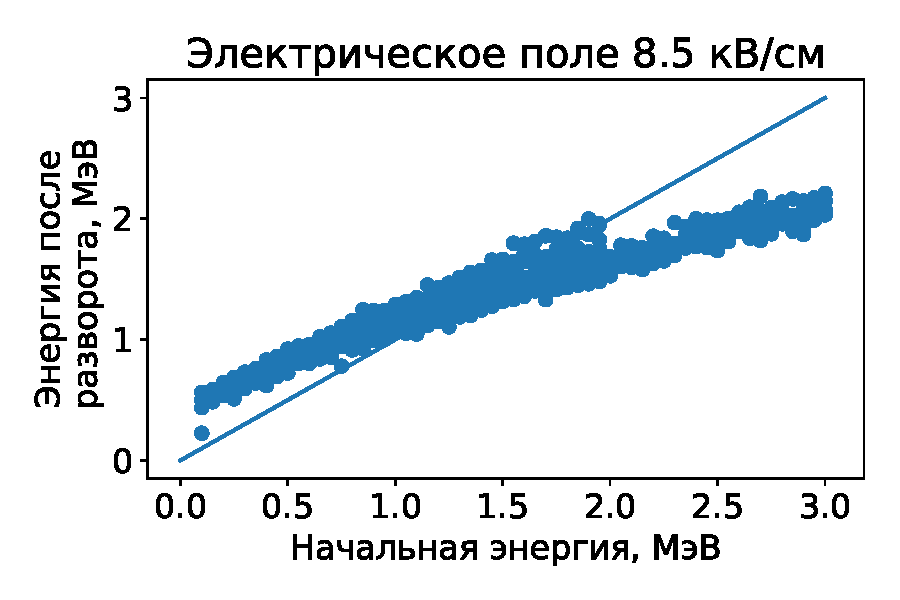
\includegraphics[width=\linewidth]{thunderstorm/rdfm/reverse_energy_8_5.pdf} \\ з)}
        \end{minipage}    
        \vfill
        \begin{minipage}[h]{0.49\linewidth}
            \center{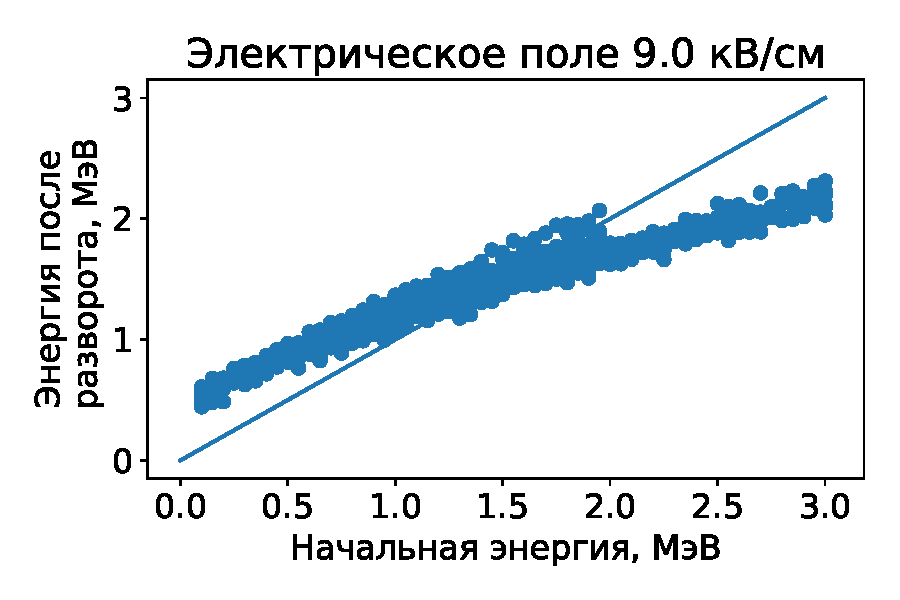
\includegraphics[width=\linewidth]{thunderstorm/rdfm/reverse_energy_9_0.pdf} \\ и)}
        \end{minipage}
        \hfill
        \begin{minipage}[h]{0.49\linewidth}
            \center{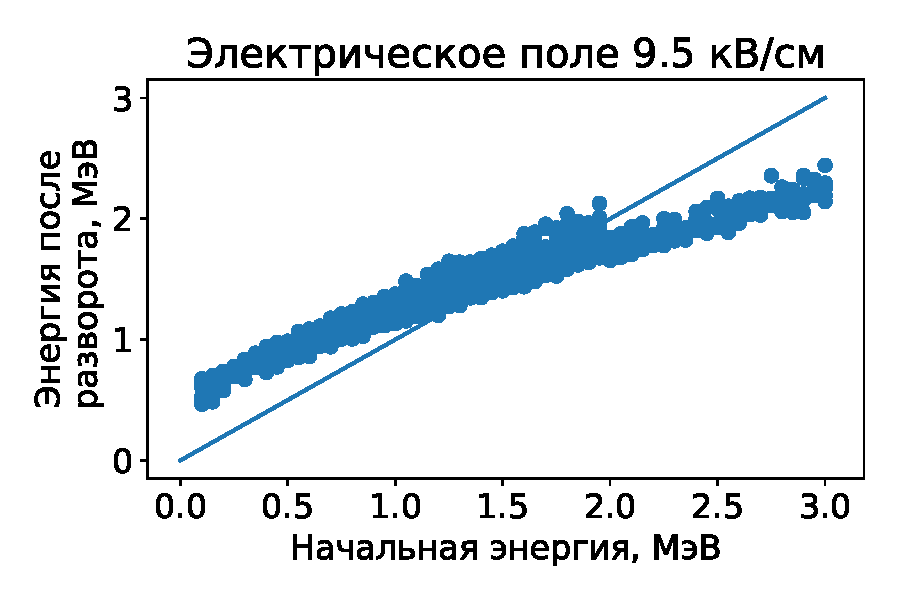
\includegraphics[width=\linewidth]{thunderstorm/rdfm/reverse_energy_9_5.pdf} \\ к)}
        \end{minipage} 
        \vfill
        \begin{minipage}[h]{0.49\linewidth}
            \center{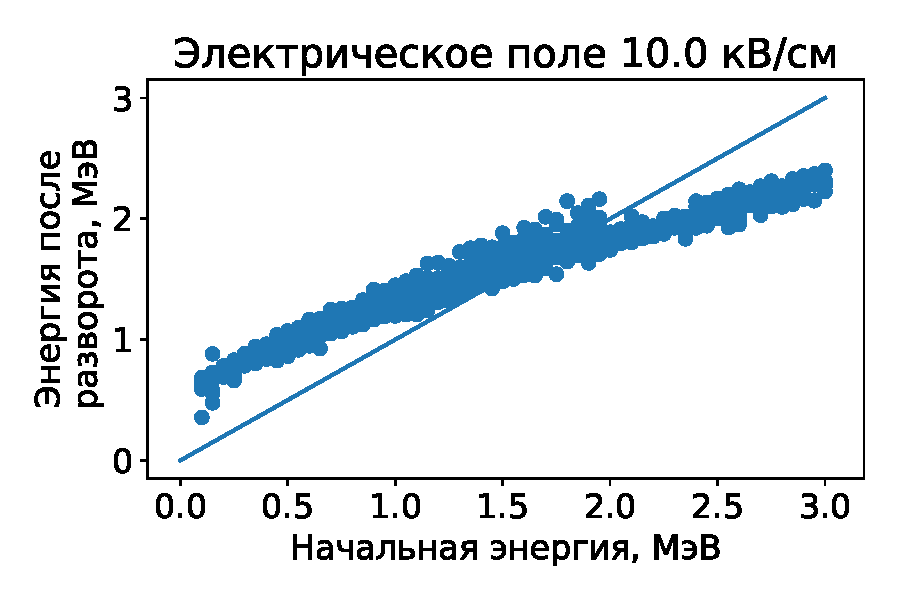
\includegraphics[width=\linewidth]{thunderstorm/rdfm/reverse_energy_10_0.pdf} \\ л)}
        \end{minipage}
        \caption{Разворот электрона}
    \end{center}
    \label{fig:storm:reverse_energy_nc_2}
\end{figure}

Результаты представлены на графиках и в таблице . Синяя линия на графике отображает результат полученный Дуаером в ~\cite{dwyer2003fundamental} при значения электрического поля и длины выше этой кривой должен наблюдаться значительный рост новых затравочных частиц ускоренный обратной связью и приводящей в возникновению TGF и ионизации облака достаточной для разряда молнии, в частности подобный результат также говорит что внутри облаков не должно быть скрытых областей с сильным полем --- подобные области должны быстро разряжаться в следствии действия механизмов обратной связи. В своей работе я взял несколько точек вдоль и чуть выше этой кривой (отмечены на графике маркером), и для данных точек провел GEANT4 моделирование в аналогичных условиях. Для каждой точки было рассчитано число новых затравочных электронов рожденных за счет гамма и позитронной обратной связи за одну итерацию на одну первичную частицу (аналогично работе~\cite{dwyer2003fundamental} электрон считался новым затравочным, если рождался в от гамма-кванта или позитрона в верхней половине облака). Число новых электронов рассчитано с учетом вероятности развернутся в электрическом поле, эта вероятность была рассчитана с помощью отдельного моделирования и показан ан графике Так же  


\begin{figure}[t]
    \begin{center}
        \begin{minipage}[h]{0.49\linewidth}
            \center{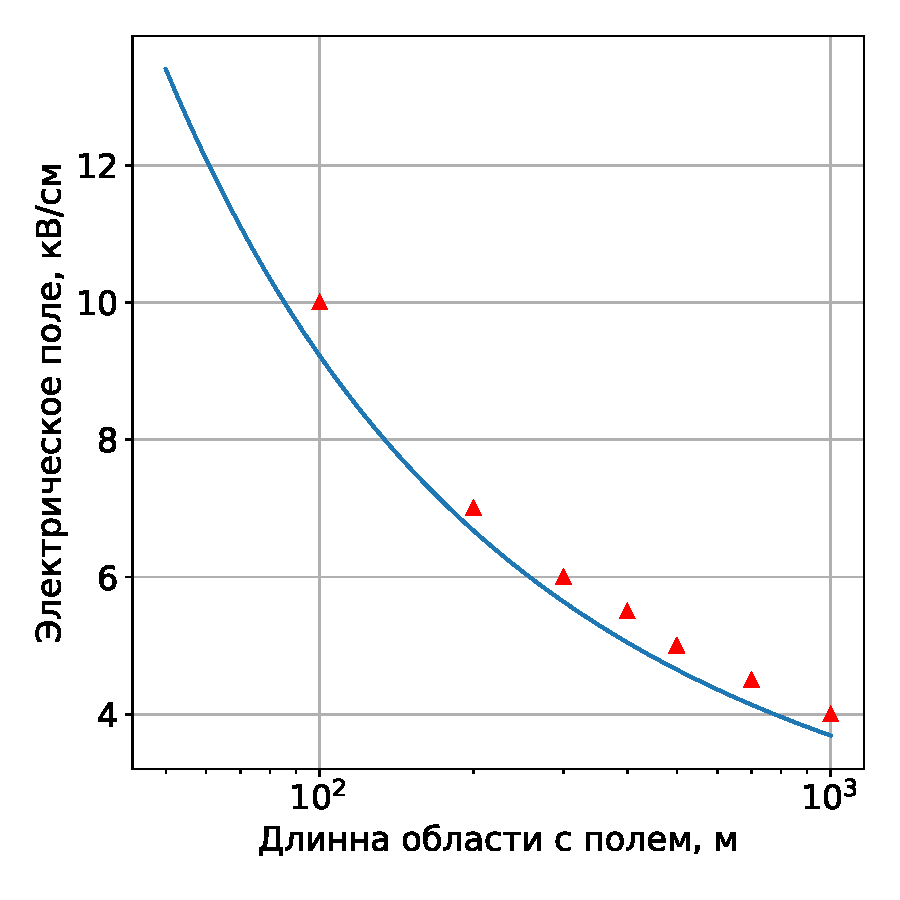
\includegraphics[width=\linewidth]{thunderstorm/rdfm/dwyer_2003.pdf} \\ а)}
        \end{minipage}
        \hfill
        \begin{minipage}[h]{0.49\linewidth}
            \center{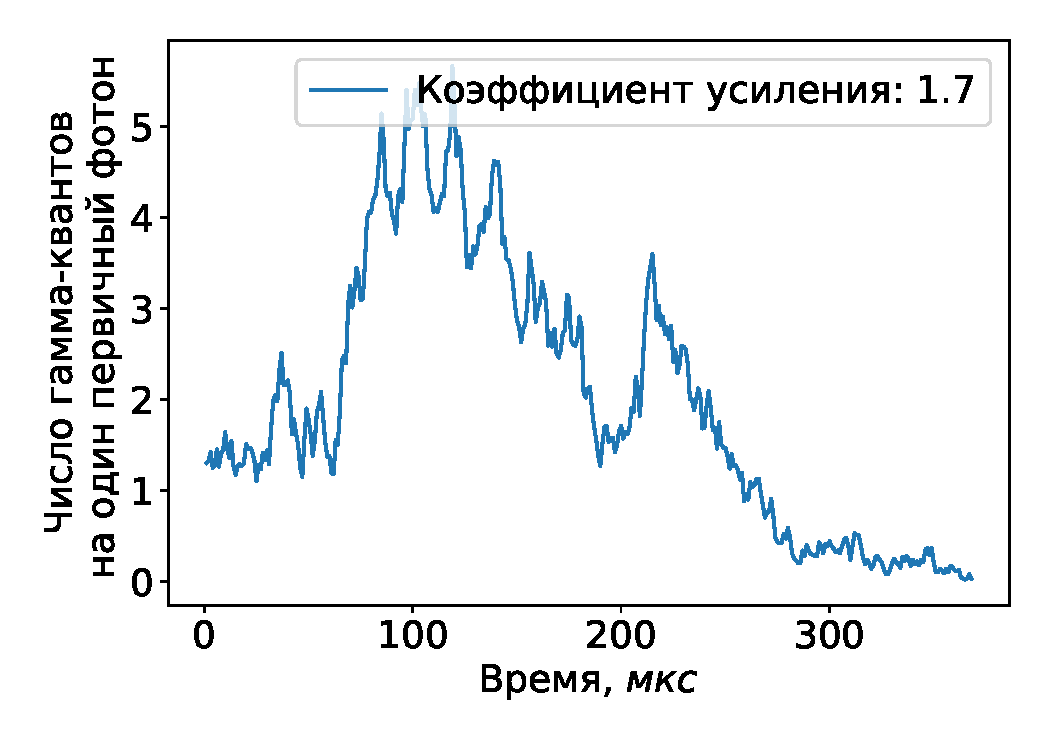
\includegraphics[width=\linewidth]{thunderstorm/RL_Extinction.pdf}   \\ б)}
        \end{minipage}
        \caption{а) Затухание лавины. б) placeholder.}
    \end{center}
    \label{fig:storm:dwyer2003}
\end{figure}

\begin{table}[h]
    \centering
    \begin{tabular}{crrrr}
        \hline
        & & & \multicolumn{2}{r}{Число новых затравочных электронов} \\
        & Поле, кВ/см &  Длина облака, м  & от гамма ОС & от позитронной ОС \\
        \hline
        & 4   &  1000&  0 & 0  \\
        & 4.5 &  700 &  200 ($\pm 10 \%$)& 400 ($\pm 5 \%$) \\
        & 5   &  500 &  100 ($\pm 14 \%$)& 40 ($\pm 5 \%$) \\
        & 5.5 &  400 &  110 ($\pm 3 \%$)& 85 ($\pm 5 \%$) \\
        & 6   &  300 &  40 ($\pm 3 \%$)& 70 ($\pm 2 \%$) \\
        & 7   &  200 &  7 ($\pm 2 \%$)& 8 ($\pm 2 \%$) \\
        & 10  &  100 &  5 ($\pm 3 \%$)& 2 ($\pm 5 \%$) \\
        \hline
    \end{tabular}
    \caption{Моделирование числа новых затравочных электронов возникающих за счет одной итерации механизма обратной связи на один первичный электрон.}
    \label{tab:storm:dwyer}
\end{table}
